\documentclass[a4paper,10pt,twocolumn]{article}
\usepackage{graphicx}
\usepackage{hyperref}
\usepackage{geometry}
\usepackage{titlesec}
\usepackage{fancyhdr}
\geometry{margin=1in}

% Define header and footer
\pagestyle{fancy}
\fancyhead[L]{\textbf{PBV1 Power Distribution Box}}
\fancyhead[R]{\today}
\fancyfoot[C]{\thepage}

\title{\textbf{Power Distribution Box for Astrophotography}\\\large Model: PBV1}
\author{Manufacturer: CoreOS}
\date{\today}

\begin{document}
\maketitle

\section*{Introduction}
\textbf{PBV1 Power Distribution Box} is designed for astrophotography setups, allowing users to efficiently power and control their astronomical equipment. It features both USB and 12V power outputs, making it an essential component for observatory automation and field setups.


\begin{center}
   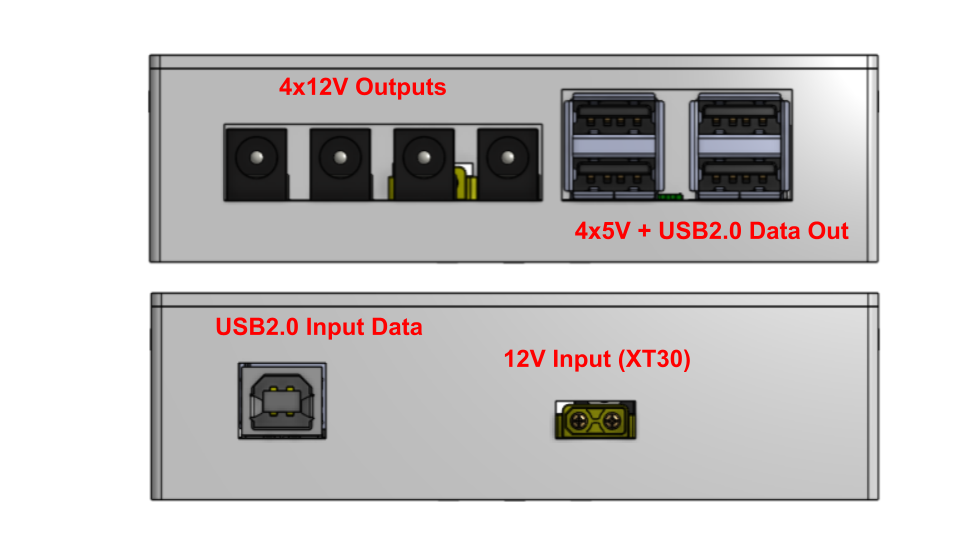
\includegraphics[width=1\columnwidth]{figures/PBV1in_outs.png} % Add image of the device
   \caption{Inputs and outputs legend }
\end{center}


\subsection*{Key Features}
\begin{itemize}
    \item 4 switchable USB 2.0 ports (3A max per port).
    \item 4 switchable 12V output ports (3A max per port).
    \item Configurable persistent output boot states .
    \item ASCOM and INDI driver support for remote control.
    \item Up to 150W of total power distribution
\end{itemize}

\section*{Technical Specifications}
\subsection*{Electrical Specifications}
\begin{table}[h]
    \centering
    \begin{tabular}{|l|l|l|l|}
    \hline
    \textbf{Specification} & Max & Typical & Min \\
    \hline
    Input Voltage (Vin) & 15V & 12V & 5V \\
    Power Consumption & 15A & - & - \\
    USB2 Ports & 4 & - & - \\
    12V Outputs & 4 & - & - \\
    \hline
    \end{tabular}
    \caption{Electrical Specifications}
\end{table}

\subsection*{Physical Specifications}
\begin{table}[h]
    \centering
    \begin{tabular}{|l|l|}
    \hline
    \textbf{Specification} & \textbf{Value} \\
    \hline
    Dimensions & 110 mm x 100 mm x 31 mm \\
    Weight & 250 grams \\
    Enclosure & Plastic (PLA thermoplastic) \\
    Mounting & Pre-drilled holes \\
    \hline
    \end{tabular}
    \caption{Physical Specifications}
\end{table}

\subsection*{Environmental Conditions}
\begin{table}[h]
    \centering
    \begin{tabular}{|l|l|}
    \hline
    \textbf{Condition} & \textbf{Range} \\
    \hline
    Operating Temperature & -10 C to 50 C \\
    Storage Temperature & -20 C to 60\ C \\
    Humidity Range & 10\%-90\% (non-condensing) \\
    \hline
    \end{tabular}
    \caption{Environmental Conditions}
\end{table}

\section*{Device Operation}
The PBV1 allows individual control of connected devices via USB and 12V outputs through serial Bluetooth communication. The outputs are managed through dedicated ASCOM and INDI (not yet released) drivers, enabling integration with astrophotography software like KStars and N.I.N.A.

\subsection*{Control Features}
\begin{itemize}
    \item Remote switch control for USB and 12V outputs.
    \item Default power states configurable via software.
    \item Real-time power monitoring (if applicable).
\end{itemize}

\section*{Setting Up PBV1 (Windows)}
\begin{enumerate}
    \item Connect the 12V XT30 connector to the PBV1.
    \item Connect a USB-A to USB-B cable between the host computer and PBV1.
    \item Ensure the computer is discoverable for Bluetooth devices.
    \item In Windows Bluetooth settings, add a new Bluetooth device.
    \item Select HC-05 and enter PIN: 1234.
    \item A new Serial Port will appear under COM and LPT in Device Manager.
    \item Note the Serial Port name (e.g., COM6) for ASCOM driver setup in NINA.
\end{enumerate}

\section*{Driver and Software Installation}
\subsection*{ASCOM Driver Installation (Windows)}
\begin{enumerate}
    \item Download the latest ASCOM driver from \url{https://drive.google.com/drive/folders/1Y-2tLgOCcrt2SNI-Vw1phUzMPFCBjFHW?usp=drive_link}.
    \item Run the installer and follow the on-screen instructions.
    \item Open astrophotography software and configure the driver by pressing the settings/options button.
    \item In the options menu, set the Serial Bluetooth port as it appears in Device Manager during PBV1 setup.
    \item You can then specify a custom label (name) for each output. The default names are Switch 1 to 8.
\end{enumerate}

\subsection*{INDI Driver Installation (Linux/Mac) (Not Released Yet)}
\begin{enumerate}
    \item Ensure INDI is installed: `sudo apt install indi-full`
    \item Start INDI and connect the device in Ekos.
\end{enumerate}

\section*{Setting Up a Custom Boot Configuration for Outputs}
\begin{enumerate}
    \item Download the BT Serial Android app from \url{https://play.google.com/store/apps/details?id=de.kai_morich.serial_bluetooth_terminal&pcampaignid=web_share} or use a desktop serial terminal (e.g., Putty).
    \item Pair your phone to the BT device and connect via a serial terminal. On a PC/laptop, connect to the BT serial port using a terminal (Baud rate: 9600).
    \item To change the boot state of a specific output, send `eX`, where `X` is 0–7 specifying the desired output port.
    \item The device will confirm that the default boot state of the specified port has changed and prompt a reboot.
    \item If changing multiple outputs, repeat step 3, then reboot the device by unplugging the power.
\end{enumerate}

\section*{Wiring \& Pinout Diagrams}
The connection diagram shown below is an example of a practical use of the PBV1 power box. 
\begin{center}
   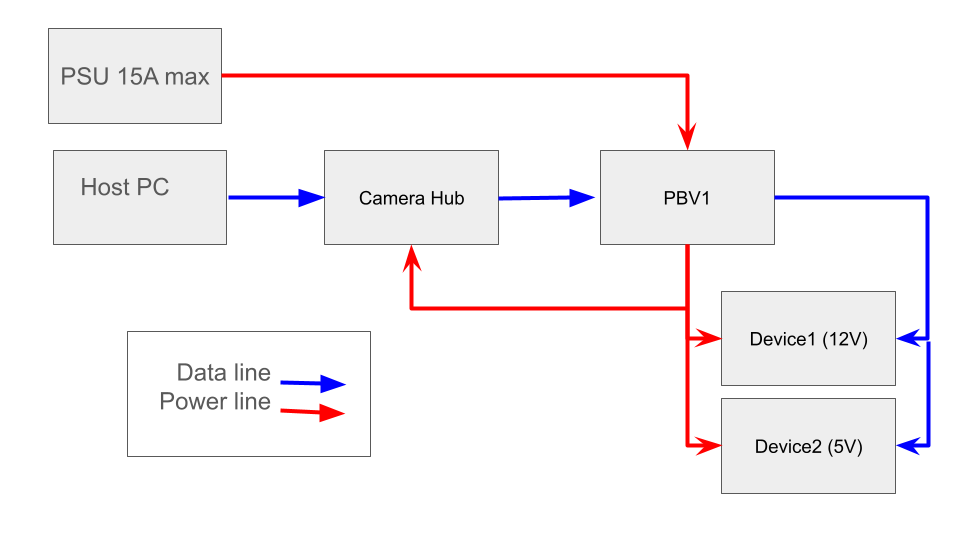
\includegraphics[width=\columnwidth]{figures/ConnectionDiagram.png} % Add wiring diagram
   \caption{Wiring diagram example}
\end{center}


\section*{Troubleshooting \& FAQs}
\textbf{Common Issues and Solutions}
\begin{itemize}
    \item \textbf{Device not detected:} Check drivers and connections.
    \item \textbf{Power output issues:} Verify fuse configuration and power source.
    \item \textbf{USB ports not working:} Try a different USB cable or check driver logs.
\end{itemize}

\section*{Warranty \& Support}
\begin{itemize}
    \item \textbf{Warranty:} There is absolutely no warranty for this device. The owner assumes full responsibility for any damage it may cause to other equipment.
    \item \textbf{Technical Support:} Limited support is provided. For critical issues, please contact \href{mailto:gcoreos@gmail.com}{this email}. Response times may vary significantly based on availability.
    \item \textbf{Knowledge page:} \url{https://drive.google.com/drive/folders/1Y-2tLgOCcrt2SNI-Vw1phUzMPFCBjFHW?usp=drive_link}.
\end{itemize}
\section*{Revision History}
\begin{table}[h]
    \centering
    \begin{tabular}{|c|c|c|}
    \hline
    Version & Date & Changes \\
    \hline
    1.0 & \today & Initial release \\
    \hline
    \end{tabular}
    \caption{Revision History}
\end{table}

\end{document}
